\subsection{Anomalous $W\gamma$ Production}
\label{sec:WgAbout_ATGC}

Most BSM physics theories predict the existence of particles which are heavier than the discovered energy range. If their masses are not accessable even by the most energetic machines, the direct detection of such particles is not possible. However, they can contribute to the productions of lower energetic particles producing loops where such heavy particles would be off-shell. The loops would give additional contributions to the process amplitude and, therefore, there would be more events produced in the process than one can expect based on the SM predictions.\\

These effects can be probed by precision measurements of the SM processes. In the electroweak sector processes of such interest include diboson and triboson productions which can occur through triple gauge couplings and quartic gauge couplings.\\ 

Triple and quartic gauge couplings (QGC) are represented by vertices with three and four bosons (Fig.~\ref{fig:TGC_and_QGC_vertices}). As discussed in Chapter~\ref{sec:WgAbout_SMEWK}, charged TGC and QGC are possible at tree level in the SM while neutral TGC and QGC are not.\\ 


\begin{figure}[htb]
  \begin{center}
    {\includegraphics[width=0.95\textwidth]{../figs/WgAbout/TGC_and_QGC_vertices.png}}
    \caption{TGC and QGC vertices}
    \label{fig:TGC_and_QGC_vertices}
  \end{center}
\end{figure}

To account for the effects from the potential loops of heavy particles, we introduce an effective Lagrangian with arbitrary values of coupling constants which can be shrinked to the SM Lagrangian if these constants would have their SM values. Such approach makes our searches model-independent because we do not specify which exactly particles form the loops but instead just check whether there is a deviation from the SM. \\

In $W\gamma$ measurement we can probe $WW\gamma$ vertex only. The most general Lorentz invariant Lagrangian of this vertex takes the following form \cite{ref_theory_aTGC}:\\

\begin{equation}\label{L_ATGC}
i L_{eff}^{WW\gamma}= i L_{eff(1)}^{WW\gamma} + i L_{eff(2)}^{WW\gamma} + i L_{eff(3)}^{WW\gamma}
\end{equation}


\begin{equation}\label{L_ATGC_1}
i L_{eff(1)}^{WW\gamma}= e [ g_1^{\gamma} A^\mu (W_{\mu\nu}^- W^{+\nu} - W_{\mu\nu}^+ W^{-\nu}) + \kappa_\gamma W_{\mu}^+ W_{\nu}^- A^{\mu\nu} + {\frac{\lambda_\gamma}{m^2_W}} A^{\mu\nu} W_\nu^{+\rho} W_{\rho\mu}^- ]
\end{equation}

\begin{equation}\label{L_ATGC_2}
i L_{eff(2)}^{WW\gamma}= e [ i g_5^\gamma \epsilon_{\mu\nu\rho\sigma}((\partial^\rho W^{-\mu})W^{+\nu} - W^{-\mu}(\partial^{\rho}W^{+\nu}))V^\sigma + i g_4^\gamma W_\mu^- W_\nu^+ (\partial^\mu A^\nu + \partial^\nu A^\mu) ]
\end{equation}

\begin{equation}\label{L_ATGC_3}
i L_{eff(3)}^{WW\gamma}= e [ \frac{\tilde{\kappa_\gamma}}{2} W_\mu^- W_\nu^+ \epsilon^{\mu\nu\rho\sigma} A_{\rho\sigma} - \frac{\tilde{\lambda_\gamma}}{2 m_W^2} W_{\rho\mu}^- W^{+\mu}_{\nu} \epsilon^{\nu\rho\alpha\beta} A_{\alpha\beta}]
\end{equation}


where $e$ is the absolute value of the electron charge, $A^\mu$ is the photon field, $W^{\pm\mu}$ are fileds of $W^\pm$ bosons, $W_{\mu\nu}=\partial_\mu W_\nu - \partial_\nu W_\mu$, $A_{\mu\nu}=\partial_\mu A_\nu - \partial_\nu A_\mu$, $m_W$ is the mass of a $W$ boson, $g_1^\gamma$, $\kappa_\gamma$, $\lambda_\gamma$, $g_5^\gamma$, $g_4^\gamma$, $\tilde{\kappa_\gamma}$, and $\tilde{\lambda_\gamma}$ are constants.\\

Despite there are~7 constants in the extended Lagrangian, only $\lambda_\gamma$ and $\kappa_\gamma$ are considered in the aTGC searches. The rest of the constants are fixed to their SM values based on various considerations. Thus, $g_1^\gamma=1$ and $g_5^\gamma=0$ are fixed to obey the electromagnatic gauge invariance for the on-shell photons. The non-zero value of $g_5^\gamma$ also violates C and P conservations, and non-zero values of $g_4^\gamma$, $\tilde{\kappa_\gamma}$, $\tilde{\lambda_\gamma}$ violate the CP conservation law. Such violation parametrizations are not considered in charged TGC measurements now but might get considered in the future.\\

The presence of aTGC would have larger effects at high energy scales. Fig.~\ref{fig:aTGC_Pt_Wg} shows these effect in $P_T^\gamma$ spectrum of 7~TeV $W\gamma \rightarrow \mu\nu\gamma$ measurement. Fig.~\ref{fig:aTGC_Pt_Examples}  shows the examples of these effects in $m_{ll}$ spectrum in 8 TeV $WW \rightarrow l\nu l\nu$ measurement (left) and $P_T^{\gamma}$ spectrum in 7 TeV $Z\gamma \rightarrow \nu\nu\gamma$ measurement (right). It is seen on the plots that aTGC spectrum at low $m_{ll}$ or low $P_T^{\gamma}$ coincides with the SM prediction but for higher $m_{ll}$ or $P_T^{\gamma}$ the disagreement becomes more significant.\\

\begin{figure}[htb]
  \begin{center}
    {\includegraphics[width=0.85\textwidth]{../figs/WgAbout/aTGC_Pt_Wg.png}}
    \caption{Distributions of $P_T^\gamma$ of simulated $W\gamma\rightarrow\mu\nu\gamma$ events with different values of aTGC constants at LHC energy of $\sqrt{s}=7$~TeV. Source of figure:  \cite{ref_Senka_thesis}.}
    \label{fig:aTGC_Pt_Wg}
  \end{center}
\end{figure}

\begin{figure}[htb]
  \begin{center}
    {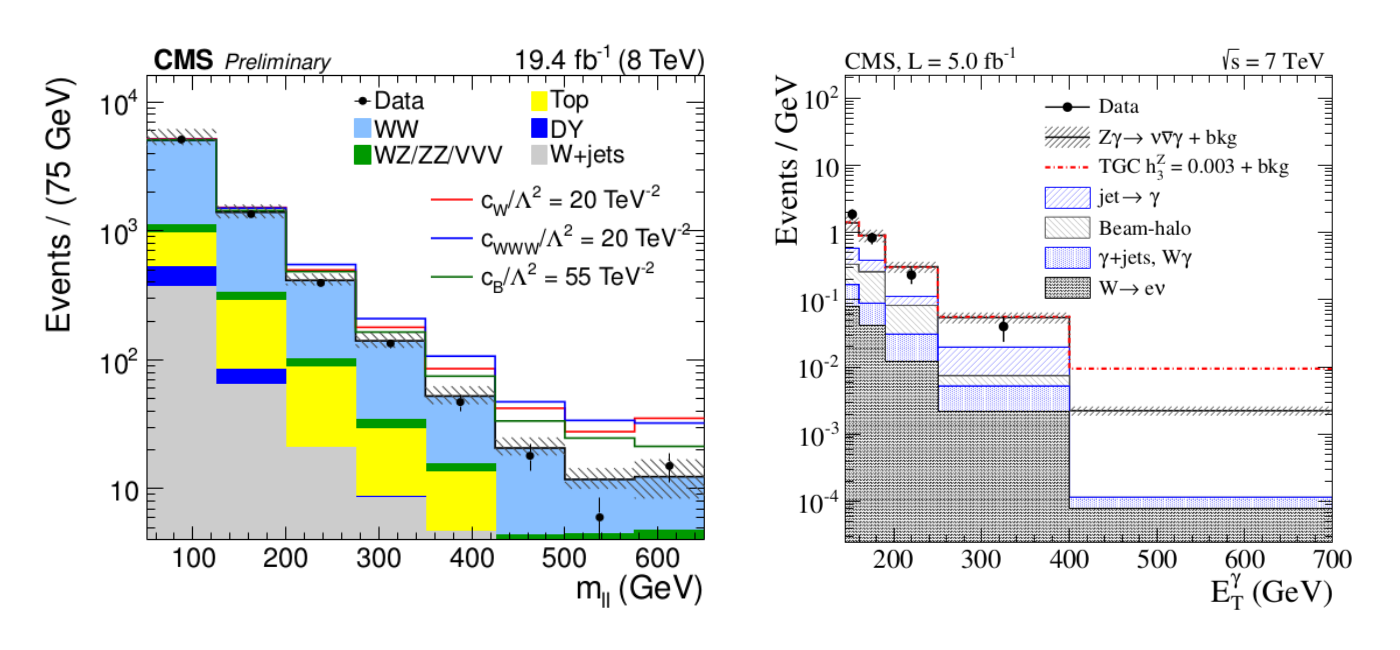
\includegraphics[width=0.85\textwidth]{../figs/WgAbout/aTGC_Pt_Examples.png}}
    \caption{Examples of the potential effects of non-zero TGC constants in $m_{ll}$ spectrum in 8 TeV $WW \rightarrow l\nu l\nu$ measurement (left) \cite{ref_CMS_8TeV_WW} and $P_T^{\gamma}$ spectrum in 7 TeV $Z\gamma \rightarrow \nu\nu\gamma$ measurement (right) \cite{ref_CMS_7TeV_Zgnunug}.}
    \label{fig:aTGC_Pt_Examples}
  \end{center}
\end{figure}



